\documentclass[11pt,twoside,a4paper]{book}  
% definice dokumentu
\usepackage[czech, english]{babel}
\usepackage[T1]{fontenc} 				% pouzije EC fonty 
\usepackage[utf8]{inputenc} 			% utf8 kódování vstupu 
\usepackage[square, numbers]{natbib}	% sazba pouzite literatury
\usepackage{indentfirst} 				% 1. odstavec jako v cestine, pro práci v aj možno zakomentovat
\usepackage{fancyhdr}					% tisk hlaviček a patiček stránek
\usepackage{nomencl} 					% umožňuje snadno definovat zkratky a jejich seznam

%%%%%%%%%%%%%%%%%%%%%%%%%%%%%%%%%%%%%%%%%%%%%%%%%%%%%%%%%%%%%%%
% informace o práci
\newcommand\WorkTitle{Analýza a návrh abstraktní vícevrstvé architektury pro práci s grafovou databází realizující metadatové úložiště pro data lineage}
\newcommand\FirstandFamilyName{Bc. Jakub Moravec}															
\newcommand\Supervisor{Ing. Michal Valenta, Ph.D.}															

\newcommand\TypeOfWork{Diplomová práce}	

\newcommand\StudProgram{Otevřená Informatika, Magisterský}	% program
\newcommand\StudBranch{Softwarové inženýrství}				% obor

%%%%%%%%%%%%%%%%%%%%%%%%%%%%%%%%%%%%%%%%%%%%%%%%%%%%%%%%%%%%%%%
% minimální importy
\usepackage{graphicx}					% pro vkládání obrázků
\usepackage{k336_thesis_macros} 		% specialni makra pro formatovani DP a BP
\usepackage[
pdftitle={\WorkTitle},				% nastaví v informacích o pdf název
pdfauthor={\FirstandFamilyName},	% nastaví v informacích o pdf autora
colorlinks=true,					% před tiskem doporučujeme nastavit na false, aby odkazy a url nebyly šedé při ČB tisku
breaklinks=true,
urlcolor=red,
citecolor=blue,
linkcolor=blue,
unicode=true,
]
{hyperref}								% pro zobrazování "prokliknutelných" linků 

% rozšiřující importy
\usepackage{listings} 			%slouží pro tisk zdrojových kódů se syntax higlighting
\usepackage{algorithmicx} 		%slouží pro zápis algoritmů
\usepackage{algpseudocode} 		%slouží pro výpis pseudokódu

%%%%%%%%%%%%%%%%%%%%%%%%%%%%%%%%%%%%%%%%%%%%%%%%%%%%%%%%%%%%%%%
% příkazy šablony
\makenomenclature								% při překladu zajistí vytvoření pracovního souboru se seznamem zkratek

\let\oldUrl\url									% url adresy budou zobrazeny: <url> 
\renewcommand\url[1]{<\texttt{\oldUrl{#1}}>}

%%%%%%%%%%%%%%%%%%%%%%%%%%%%%%%%%%%%%%%%%%%%%%%%%%%%%%%%%%%%%%%
% vaše vlastní příkazy
\newcommand*{\nomExpl}[2]{#2 (#1)\nomenclature{#1}{#2}} 	% usnadňuje zápis zkratek : Slova ke Zkrácení (SZ)
\newcommand*{\nom}[2]{#1\nomenclature{#1}{#2}} 			% usnadňuje zápis zkratek : SZ



%%%%%%%%%%%%%%%%%%%%%%%%%%%%%%%%%%%%%%%%%%%%%%%%%%%%%%%%%%%%%%%
% vlastní dokument
%%%%%%%%%%%%%%%%%%%%%%%%%%%%%%%%%%%%%%%%%%%%%%%%%%%%%%%%%%%%%%%
\begin{document}
	
	%%%%%%%%%%%%%%%%%%%%%%%%%% 
	% nastavení jazyka, kterým je práce psána
	\selectlanguage{czech}	% podle jazyka práce nastavte na [czech | english]
	\translate				% nastaví české nebo anglické popisy (např. katedra -> department); viz k336_thesis_macros

	%%%%%%%%%%%%%%%%%%%%%%%%%%    
	% Poznamky ke kompletaci prace
	% Nasledujici pasaz uzavrenou v {} ve sve praci samozrejme 
	% zakomentujte nebo odstrante. 
	% Ve vysledne svazane praci bude nahrazena skutecnym 
	% oficialnim zadanim vasi prace.
	{
	\pagenumbering{roman} \cleardoublepage \thispagestyle{empty}
	\chapter*{Na tomto místě bude oficiální zadání vaší práce}
	\begin{itemize}
		\item Toto zadání je podepsané děkanem a vedoucím katedry,
		\item musíte si ho vyzvednout na studijním oddělení Katedry počítačů na Karlově náměstí,
		\item v jedné odevzdané práci bude originál tohoto zadání (originál zůstává po obhajobě na katedře),
		\item ve druhé bude na stejném místě neověřená kopie tohoto dokumentu (tato se vám vrátí po obhajobě).
	\end{itemize}
	\newpage
	}

	%%%%%%%%%%%%%%%%%%%%%%%%%%    
	% Titulni stranka / Title page 
	\coverpagestarts

	%%%%%%%%%%%%%%%%%%%%%%%%%%%    
	% Poděkovani / Acknowledgements 

	\acknowledgements
	\noindent
	Zde můžete napsat své poděkování, pokud chcete a máte komu děkovat.


	%%%%%%%%%%%%%%%%%%%%%%%%%%%   
	% Prohlášení / Declaration 

	\declaration{V~Kořenovicích nad Bečvárkou dne 15.\,5.\,2008}
	%\declaration{In Kořenovice nad Bečvárkou on May 15, 2008}


	%%%%%%%%%%%%%%%%%%%%%%%%%%%%    
	% Abstrakt / Abstract 
 
	\abstractpage

	Translation of Czech abstract into English.

	\vglue60mm

	\noindent{\Huge \textbf{Abstrakt}}
	\vskip 2.75\baselineskip

	\noindent
	Abstrakt práce by měl velmi stručně vystihovat její obsah. Tedy čím se práce zabývá a co je jejím výsledkem/přínosem.

	\noindent
	Očekávají se cca 1 -- 2 odstavce, maximálně půl stránky.

	%%%%%%%%%%%%%%%%%%%%%%%%%%    
	% obsahy a seznamy
	\tableofcontents		% Obsah / Table of Contents 

	% pokud v práci nejsou obrázky nebo tabulky - odstraňte jejich seznam
	\listoffigures			% Obsah / Table of Contents 
	\listoftables			% Seznam tabulek / List of Tables

	%%%%%%%%%%%%%%%%%%%%%%%%%% 
	% začátek textu  
	\mainbodystarts

\chapter{Úvod}
\label{sec:uvod}
\section{Data lineage}

% Úvod
Data a z nich získávané informace vždy byly v centru pozornosti informačních technologií a jejich význam každým rokem stoupá. V digitální podobě jsou dnes zakódovány takřka všechny informace včetně našich osobních údajů, bankonvních transakcí, či zdravotních informací. Zároveň stále roste roste množství těchto dat\footnote{Podle statistiky IDC \cite{Idc14} se celkový objem dat virtuálního světa zdvojnásobuje každé dva roky.}.
Je tedy kladena velká pozornost na procesy, kterými jsou data zpracovávána a pomocí kterých jsou z dat získávány informace. Existuje několik přístupů k tomuto problému, ať už se jedná o tradiční relační databázové systémy, datové sklady a \textit{\nomExpl{OLAP}{Online Analytical Processing}} analytické nástroje, \textit{data miningové} technologie, nebo novější obory, jako jsou \textit{NoSQL} databáze a analytické nástroje. Ať už je zvolen kterýkoliv z těchto přístupů, procesy zpracovávající data bývají komplexní a často ne zcela intuitivní pro samotné vývojáři, natož potom pro analytiky či dokonce byznys uživatele.

% Data Lineage
Do popředí se tak dostává nová skupina nástrojů označovaných jako Data lineage.\footnote{Stejně jako mnoho další termínů z oblasti informačních technologií se Data lineage nepřekládá, nebudeme ho tedy překládat ani my. Pokud bychom termín však přeci jen chtěli popsat českými slovy, nejvhodnější překlad by byl zřejmě "řízení datových toků".}
Jejich cílem je analyzovat end-to-end datové toky v systému - zdroje, transformace a cíle dat a pomocí této analýzy umožnit uživateli vhled do tohoto procesu. To může být velmi komplexní úkol, informační systém se typicky skládá z řady navzájem propojených technologií, a nástroj pro analýzu Data lineage si musí umět poradit nejen s každým z nich separátně, ale také s případnými transformacemi na hranicích těchto systémů.

% Manta Flow
Jedním z úspěšných nástrojů pro Data lineage je \textit{Manta Flow}\footnote{\url{https://getmanta.com/}}. Nástroj analyzuje zdrojové kódy vybraných RDBMS databází, Big Data nástrojů a ETL nástrojů.
Zdrojové kódy analyzovaných systémů jsou pravidelně parsovány dle syntaktických a sémantických pravidel podporovaných nástrojů a následně jsou analyzovány přímé a nepřímé\footnote{Představme si relační databázi s tabulkami \textit{A}, \textit{B} a \textit{C}. Představme si, že data z tabulky \textit{A} jsou \textit{ETL transformací} přenesena do tabulku \textit{B}. Tato \textit{ETL transformace} filtruje data z tabulky \textit{A} dle dat z tabulky \textit{C}. Potom z tabulky \textit{A} do tabulky \textit{B} vede \textit{přímý datový tok} a z tabulky \textit{C} do tabulky \textit{B} vede \textit{nepřímý datový tok}.} datové toky a transformace dat v informačním systému.
Získané informace jsou ukládány do metadatového uložiště, jímž je v současné době grafová databáze \textit{Titan}\footnote{\url{http://titan.thinkaurelius.com/}}. Klientská část aplikace potom umožňuje uživateli vizualizovat datové toky dle zadaných parametrů (zdroj a cíl datového toku, úroveň abstrakce atd.). Dynamicky tak vznikají komplexní dotazy do metadatové databáze, pomocí kterých jsou procházeny grafy datových toků a vraceny výsledky.

\section{Definice problému}
% Neexistence standardů GDB
Přestože má použití grafové databáze jako metadatového uložiště pro Data lineage nástroje silné opodstatnění\footnote{Grafová databáze umožňuje výrazně rychlejší hledání datových toků v informačních systémech, než by umožňovali jiné architektury. Způsob procházení grafů je popsán v kapitole \ref{sec:gdb-dotazy}.}, přináší s sebou krom nesporných výhod také řadu problémů. Jejich společným jmenovatelem je fakt, že v oblasti grafových databází, která je relativně nová a stále prochází dynamickým rozvojem, nejsou zatím jasně definovány obecně podporované standardy. Neexistuje například univerzální, stabilní a obecně podporovaný dotazovací jazyk pro grafové databáze (například v oblasti relačních databází tuto úlohu plní SQL). To vede mimo jiné k tomu, že nejsou v tuto chvíli definovány doporučené postupy softwarového inženýrství pro tvorbu abstraktních rozhraní pracujících s grafovými databázemi. Není tak překvapaním, že je při používání grafových databází v aplikacích často míchána perzistentní a byznys logika aplikace, což je typickou ukázkou špatného návrhu\cite{Taylor09}. Pro produkt \textit{Manta Flow} je tento problém velice aktuální - používaná databáze \textit{Titan} již není dále vyvýjena, brzy skončí její podpora \cite{Titan04} a je pravděpodobné, že dojde k její výměně za jinou technologii. Cílem této práce je navrhnout abstraktní architekturu pro práci s grafovou databází, která bude vyhovovat potřebám nástroje \textit{Manta Flow} a bude v co největší míře oddělovat perzistentní logiku od zbytku aplikace. Zavedení této vrstvy aplikace bude pravděpodobně znamenat zásah do celé architektury aplikace. Součástí práce tedy musí být nový návrh architektury aplikace reflektující změnu v přístupu ke grafové databází.

\section{Struktura diplomové práce}
Práce je rozdělena na teoretickou a experimentální část.

% Teorietická část
Cílem teoretické části je popsat obecné principy grafových databází, jejich vnitřní organizaci a možnosti dotazování dat. Dále jsou popsány možnosti abstrakce ve světě softwarového inženýrství - ať už na úrovní procesů a programových rozhraní (API), nebo na nižších úrovních - například návrhových vzorů.

%Experimentální část
Experimentální část práce obsahuje hlubší analýzu potřeb projektu \textit{Manta Flow} pro přístup ke grafové databázi. Na základě teoretické části práce je navržena vícevrstvá abstraktní architektura, vytvořeno \nomExpl{PoC}{Proof of Concept} řešní a to otestováno nad reálnými data.




%%%%%%%%%%%%%%%%%%%%%%%%%% 
% Seznam literatury je v samostatnem souboru reference.bib. Ten
% upravte dle vlastnich potreb, potom zpracujte (a do textu
% zapracujte) pomoci prikazu bibtex a nasledne pdflatex (nebo
% latex). Druhy z nich alespon 2x, aby se poresily odkazy.

% originally following specification for bibliography formating was used
%\bibliographystyle{abbrv}

% Here is an improvment by Petr Dlouhy (April 2010).
% It is mainly for supervisors who expect Czech fomrating rules for references
% Additional feature is live url addresses to sources from your pdf file
% It requires the file csplainnat.bst (included in this sample zipfile).

\bibliographystyle{csplainnat}

%bibliographystyle{plain}
%\bibliographystyle{psc}
{
%JZ: 11.12.2008 Kdo chce mit v techto ukazkovych odkazech take odkaz na CSTeX:
\def\CS{$\cal C\kern-0.1667em\lower.5ex\hbox{$\cal S$}\kern-0.075em $}
\bibliography{reference}
}

% M. Dušek radi:
%\bibliographystyle{alpha}
% kdy citace ma tvar [AutorRok] (napriklad [Cook97]). Sice to asi neni  podle ceske normy (BTW BibTeX stejne neodpovida ceske norme), ale je to nejprehlednejsi.
% 3.5.2009 JZ polemizuje: BibTeX neobvinujte, napiste a poskytnete nam styl (.bst) splnujici citacni normu CSN/ISO.


%%%%%%%%%%%%%%%%%%%%%%%%%% 
% vše co následuje bude uvedeno v přílohách
\appendix	

\printnomenclature
\label{apx:zkratky}

\chapter{Obsah přiloženého CD}
\textbf{\large Tato příloha je povinná pro každou práci. Každá práce musí totiž obsahovat přiložené CD. Viz dále.}

Může vypadat například takto. Váš seznam samozřejmě bude odpovídat typu vaší práce. (viz \cite{infodp}):

\begin{figure}[h]
\begin{center}
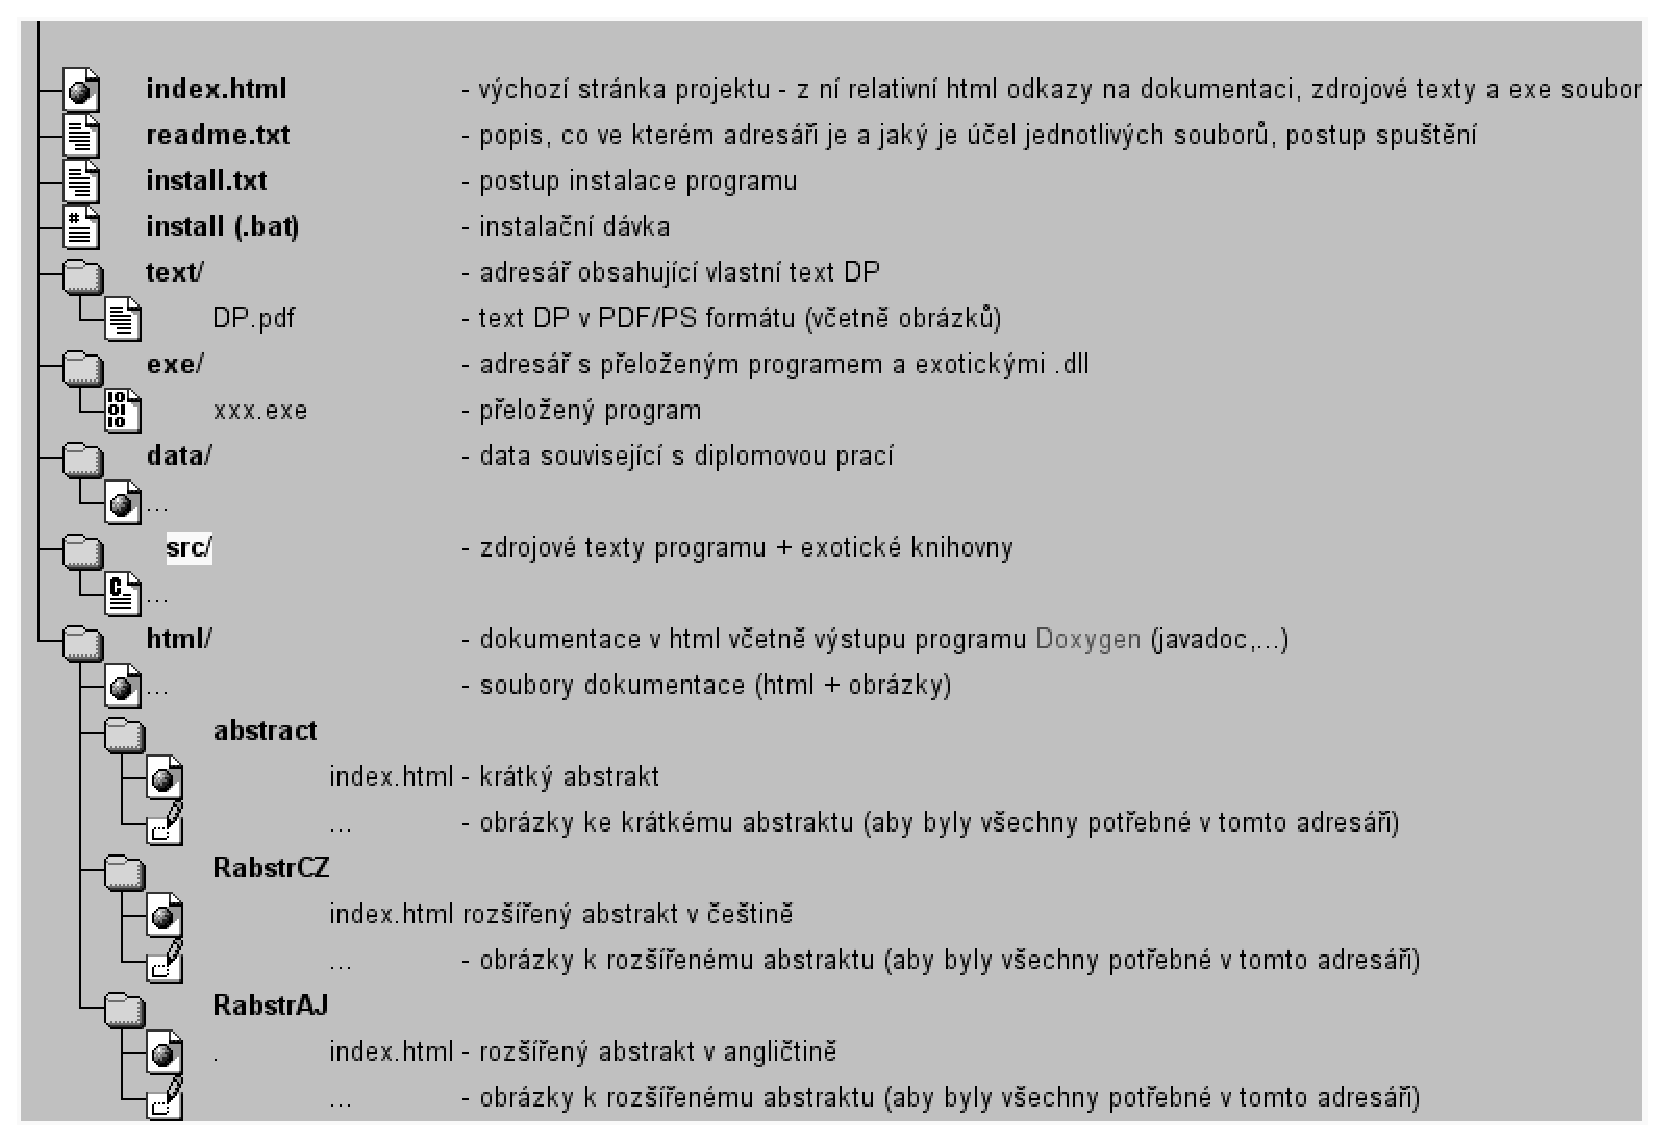
\includegraphics[width=14cm]{figures/seznamcd}
\caption{Seznam přiloženého CD --- příklad}
\label{fig:seznamcd}
\end{center}
\end{figure}

Na GNU/Linuxu si strukturu přiloženého CD můžete snadno vyrobit příkazem:\\ 
\verb|$ tree . >tree.txt|\\
Ve vzniklém souboru pak stačí pouze doplnit komentáře.

Z \textbf{README.TXT} (případne index.html apod.)  musí být rovněž zřejmé, jak programy instalovat, spouštět a jaké požadavky mají tyto programy na hardware.

Adresář \textbf{text}  musí obsahovat soubor s vlastním textem práce v PDF nebo PS formátu, který bude později použit pro prezentaci diplomové práce na WWW.

\end{document}
